\documentclass{beamer}
\usepackage{beamerthemeshadow}
\usepackage{graphicx}
\usepackage{color}
\usepackage[utf8]{inputenc}
\usepackage{hyperref}
\usepackage[flushleft]{threeparttable}
\definecolor{beamer@darkred}{rgb}{0.75,0.5,0.1}
\setbeamercolor{structure}{fg=beamer@darkred}

\def\d{{\fontencoding{T1}\selectfont\dj}}
\def\D{{\fontencoding{T1}\selectfont\DJ}}


\title{Tehničko i naučno pisanje}
\subtitle{-- Tehnološka Singularnost --}
\author{Nikola Ahac, Dimitrije Petroonijević, Mladen Radojević, Lazar Stošić}
\institute{Matematički fakultet\\Univerzitet u Beogradu}
\date{
	\footnotesize{Beograd, 2022.}	
}

\begin{document}
\begin{frame}
	\thispagestyle{empty}
	\titlepage
\end{frame}

\addtocounter{framenumber}{-1}

\begin{frame}[fragile]\frametitle{Literatura}
	\begin{itemize}
		\item Zasnovano na:\\
		The Technological Singularity, Murray Shanahan.
	\end{itemize}
\end{frame}

\begin{frame}
	\frametitle{Pregled} % Table of contents slide, comment this block out to remove it
	\tableofcontents[hidesubsections] 
\end{frame}

\section{Verovatnoća}

\begin{frame}[fragile]\frametitle{Verovatnoća da će doći do singularnosti}
    \begin{itemize}	
        \item Glavni faktori:
        \begin{itemize}	
            \item Poboljšivači inteligencije
            \item Otežavanje tehnološkog napretka
            \item Eventualna fizička granica
      \end{itemize}
    \end{itemize}
\end{frame}

\begin{frame}[fragile]\frametitle{Razvoj brzine tehnološkog napretka}
    \begin{itemize}	
        \item Murov zakon (eng. Moore's Law)
        \item Kurcvailov zakon o ubrzanom povratku
    \end{itemize}
    \begin{figure}[h!]
        \centering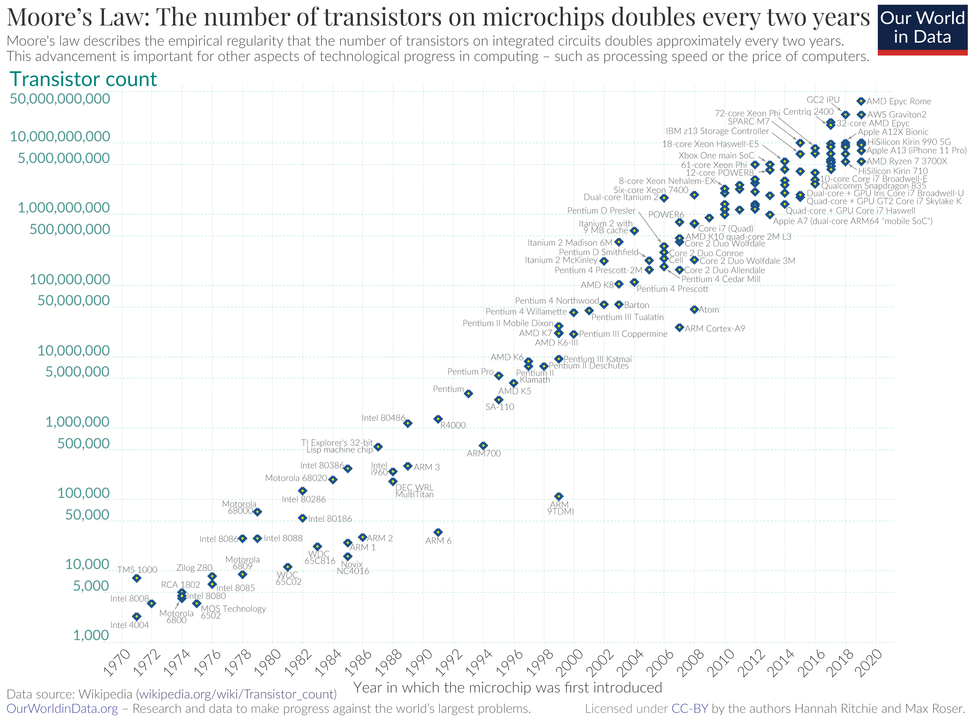
\includegraphics[height=5cm]{moore.png} 
        \caption{Grafik Murovog zakon}
        \label{fig:murovzakon}
    \end{figure}
\end{frame}


\begin{frame}[fragile]\frametitle{Razvoj algoritama}
    \begin{itemize}	
        \item Kako se razlikuje od čistog povećanja brzine izvršavanja?
        \item "Seed AI"
    \end{itemize}
\end{frame}

\section{Zakljucak}

\begin{frame}[fragile]\frametitle{Kako ljudi uče?}
	\begin{itemize}	
		\item Ljudi ne komuniciraju samo rečima. Prema nekim
		istraživanjima:
		\begin{itemize}
			\item samo 8\% poruke se prenese samim rečima (verbalna komunikacija)
			\item 37\% se prenesi bojom glasa, tonalitetom, pauzama u govoru (paralingvističkim znakovima)
			\item 55\% poruke se prenosi govorom tela: pratećim pokretima, izrazom lica i
			očiju, stavom tela i drugo (neverbalna komunikacija)
		\end{itemize}
		\item Verbalnim putem se najčešće prenose činjenice i
		sirove informacije, dok se neverbalnim putem prenose stavovi i
		emocionalni odnos prema činjenicama koje izlažemo.
	\end{itemize}
\end{frame}

\end{document}
